\chapter{Self-testing of the two-qubit maximally entangled state}

Two-qubit maximally entangled states are relevant to a few quantum information processing tasks.
In this chapter we study the self-tests of such a state.

\medbreak 

We consider a variation of a Bell game where Alice and Bob receive copies of an unknown state $\rho_{AB} \in \mathcal{L}(\mathscr{H}^A \otimes \mathscr{H}^B)$ from an unknown source.
Alice has access to the subsytem that lays in the Hilbert space $\mathscr{H}^A$ while Bob has access to the one in $\mathscr{H}^B$, both of unknown dimension.
To ease calculations, we can purify this shared state, without loss of generalities. 
Introducing the purification space $\Hil^C$, we have the pure state $\ket{\psi_{ABC}}\in \Hil^A \otimes \Hil^B \otimes \Hil^C$ which satisfies $\tr_C \left[\ket{\psi_{ABC}}\bra{\psi_{ABC}}\right] = \rho_{AB}$.

Each party has a measurement device with two inputs, $x,y=\{0,1\}$, respectively corresponding to observables $A_x$ acting on $\mathscr{H}^A$, for Alice, and $B_y$ on $\mathscr{H}^B$, for Bob.
These measurements only have two possible outcomes $(a,b)=\pm1$.
From this Bell game, Alice and Bob will construct the correlation $P$ from the individual probabilities $p(ab|xy)$, and from which we want to certify that $\rho_{AB}$ is a two-qubit maximally entangled state $\ket{\psi^{\text{target}}_{AB}}$.

Formally, a self-testing statement can be derived if for all the \textit{quantum realization} $\{\psi_{ABC},A_x,B_y\}$ compatible with the observed correlation $P$, there exists a local isometry $\Lambda = \Lambda_A \otimes \Lambda_B \otimes \id_C$ satisfying
\begin{equation}
	\Lambda [ \ket{00}_{A'B'} \otimes \ket{\psi}_{ABC}] = \ket{\psi^\text{target}_{A'B'}} \otimes \ket{\text{junk}}_{ABC}
	\label{eq:self-testing_statement}
\end{equation}
where $A'$ and $B'$ are ancilliary systems belonging respectively to Alice and Bob, that are used to \textit{extract} the target state.
The rest of this chapter explains how to obtain this statement for two-qubit maximally entangled states.

\medbreak

As stated in the previous chapter, the \acrshort{chsh} inequality 
\begin{equation}
	S = \left | \mean{A_0 B_0} + \mean{A_0 B_1} + \mean{A_1 B_0} - \mean{A_1 B_1}  \right | \leq 2
\end{equation}
is maximally violated for a \acrshort{chsh} score of $2\sqrt{2}$, and such a score can be obtain from a maximally entangled two-qubit state and anticommuting measurements. 
Conversely, it was proven that a score of $2\sqrt{2}$ can only be reached by a maximally entangled state, and for anticommuting measurements~\cite{Summers1987,Popescu92,Tsirelson1993}. 
Therefore, we can construct a formal self-testing statement from correlations yielding a maximal \acrshort{chsh} score.

\medbreak

Let us first derive some useful properties on the involved measurements.

As written in the previous part, the probability to obtain outcomes $a,b$ from inputs $x,y$ is given by the Born rule, as in ~\refeq{Born}. 
From the state obtained after purification, these probabilities are
\begin{equation}
	p(ab|xy) = \bra{\psi_{ABC}} M^a_x \otimes M^b_y \otimes \id_C \ket{\psi_{ABC}}
\end{equation}
where $\id_C$ is the identity operator on the purification space, and with the \acrshort{povm} elements $M^a_x$ for Alice and $M^b_y$ for Bob satisfying
\begin{equation}
	\begin{split}
		M^{a}_x \succeq 0 \quad \forall\,a,x, &\qquad \sum_a M^a_x = \id \quad \forall\,x\, ,\\
		M^{b}_y \succeq 0 \quad \forall\,b,y, &\qquad \sum_b M^b_y = \id \quad \forall\,y\, .
	\end{split}
\end{equation}
Alice and Bob observables can be reconstructed from the \acrshort{povm} following
\begin{equation}
	\begin{split}
		\tilde{A}_x &= \sum_a \,a M^a_x = M^{+1}_x - M^{-1}_x, \\
		\tilde{B}_y &= \sum_b \,b M^b_y = M^{+1}_y - M^{-1}_y.
	\end{split}	
\end{equation}
From this construction and the properties of \acrshort{povm}s, we can deduce that the observables $\tilde{A}_x$ and $\tilde{B}_y$ are unitary and Hermitian.
Since we can always assume the measurements of Alice and Bob to act trivially on the extra subsystem, Alice's observables are defined as $A_x = (\tilde{A}_x \otimes \id_C)$ and similarly for Bob, $B_y=(\tilde{B}_y \otimes \id_C)$. 
Note that $A_x$ and $B_y$ are also Hermitian and unitary.
 
\medbreak

We can now prove the anticommuting nature of the measurements.
First, we introduce the shifted CHSH operator, $2\sqrt{2}\id-\mathcal{B}_\text{CHSH}$, where $\mathcal{B}_\text{CHSH}$ is the CHSH operator defined in \refeq{CHSH_operator}. 
This operator admits the following sum-of-squares~\cite{Pironio2010} decomposition 
\begin{equation}
	\begin{split}
		2&\sqrt{2}\id-\mathcal{B}_\text{CHSH} = \\
		\frac{1}{\sqrt{2}}&\left[ \left(\id_A \otimes \frac{B_0+B_1}{\sqrt{2}} - A_0 \otimes \id_B \right)^2 
		+ \left( \id_A \otimes \frac{ B_0-B_1}{\sqrt{2}} - A_1\otimes \id_B \right)^2 \right].
	\end{split}
\end{equation}
Any state $\ket{\psi}$ leading to a maximal CHSH violation, i.e. $\bra{\psi}\mathcal{B}_\text{CHSH}\ket{\psi}=2\sqrt{2}$, implies
\begin{equation}
	\bra{\psi}\left(2\sqrt{2}\id-\mathcal{B}_\text{CHSH}\right)\ket{\psi} = 0
\end{equation}
which is only satisfy if
\begin{equation}
	\begin{split}
		\bra{\psi} \left(\id_A \otimes \frac{B_0+B_1}{\sqrt{2}} - A_0\otimes \id_B \right)\ket{\psi} &= 0,  \\
		\bra{\psi} \left(\id_A \otimes \frac{B_0-B_1}{\sqrt{2}} - A_1\otimes \id_B \right)\ket{\psi} &= 0 
	\end{split}
\end{equation}
from which we can deduce the relations
\begin{equation}
	\begin{split}
		\left(\id_A \otimes \frac{B_0+B_1}{\sqrt{2}}\right)\ket{\psi} &=  (A_0\otimes \id_B)\ket{\psi}, \\
		\left(\id_A \otimes \frac{B_0-B_1}{\sqrt{2}}\right)\ket{\psi} &=  (A_1\otimes \id_B)\ket{\psi}.
	\end{split}	
	\label{eq:aliceBobMeasEquivalence}
\end{equation}
From the last two relations, we can prove the anticommuting nature of the measurement on the support of $\ket{\psi}$ following
\begin{equation}
	\begin{split}
		&\{A_0 \otimes \id_B,A_1 \otimes \id_B\} \ket{\psi} \\
		& = \left((A_0 A_1 \otimes \id_B)+(A_1 A_0 \otimes \id_B)\right)\ket{\psi}  \\
		& = \left(\frac{(\id_A \otimes (B_0+B_1)(B_0-B_1)) + (\id_A \otimes (B_0-B_1)(B_0+B_1)}{2}\right)\ket{\psi} \\
		& = 0.
	\end{split}
	\label{eq:anticommuting}
\end{equation}
From the symmetric properties of the correlation, the same anti-commutation relation can be infer for Alice's measurements.

\medbreak

To construct a self-testing statement we now need to explicitly build the local isometry $\Lambda$. 
Intuitively, from \refeq{self-testing_statement}, the isometry transfers the relevant degree of freedom of $\ket{\psi_{ABC}}$ into the parties ancilliary systems.
This can be build from \textit{SWAP} operations, each transferring information from a register to another.
If constructing local isometry from SWAP operations is mentioned in the original self-testing manuscript for the self-test of two-qubit maximally entangled states~\cite{Mayers2004}, it was then generalized to other states and to robust self-testing in \cite{McKague2012,Yang2014,Bancal15}. 

To better grasp the construction of the SWAP isometry, we fix the target two-qubit maximally entangled state to be the singlet $\ket{\psi^-}=\frac{\ket{01}-\ket{10}}{\sqrt{2}}$.
If the shared state is the target state, the local isometry should act as follow
\begin{equation}
	\Lambda[\ket{00}_{A'B'} \otimes \ket{\psi^-}_{AB}] = \ket{\psi^-}_{A'B'} \otimes \ket{junk}_{AB}.
\end{equation}
This can be achieve with the circuit depicted in \reffig{swap} with the Hadamard gate $H=(\sigma_x+\sigma_z)/\sqrt{2}$ and where $Z_A=Z_B=\sigma_z$ and $X_A=X_B=\sigma_x$.
As we are in a device-independent framework, this construction has to be made solely from the information we previously derived.

\begin{figure}
	\begin{center}
		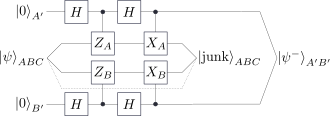
\includegraphics[width=0.95\textwidth]{chapters/selftesting/img/swap.pdf}
	\end{center}
	\caption{Circuit representation of the isometry $\Lambda$.}
	\label{fig:swap}
\end{figure}

First, we build the operators $X$ and $Z$ from Alice and Bob's observables
\begin{equation}
	\begin{split}
		Z_A = A_0, \qquad &X_A = A_1, \\
		Z_B = \frac{B_0 - B_1}{\sqrt{2}}, \qquad &X_B = \frac{B_0 + B_1}{\sqrt{2}}. \\ 
	\end{split}
\end{equation}
For $\Lambda$ to be a physical isometry, these operators have to be Hermitian and unitary.
Since we know that $A_x,B_y$ are Hermitian, and given that the sum of Hermitian matrices are Hermitian, our operators are Hermitian.
Trivially, $Z_A$ and $X_A$ are unitary. 
However, this is not the case for $Z_B$ and $X_B$, we need to \textit{regularise} them.
As detailed in \cite{Supic2019}, from an Hermitian operator $O$, we build an operator $O^\star$ by changing all the zero eigenvalues of $O$ to $1$, from which we construct a unitary operator $O'$ following $O'=|O^\star|^{-1} O^\star$.
Thanks to \refeq{aliceBobMeasEquivalence}, we can show that $Z_B'$ and $X_B'$ act the same way as $Z_B$ and $X_B$ on any state $\ket{\psi}$ following
\begin{equation}
	\begin{split}
		||(O_B' - O_B) \ket{\psi}|| &= ||(\id - O_B^\dag O_B)\psi|| \\
									&= ||(\id-|O_B|)\ket{\psi}|| \\
									&= ||(\id-|O_A O_B|)\ket{\psi}|| \\
									&\leq ||(\id-O_A O_B)\ket{\psi}|| \\
									&= 0
	\end{split}
\end{equation}
where $O$ can be replaced by either $X$ or $Z$.

We can now compute the effect of the isometry on the shared system and the ancillas
\begin{equation}
	\begin{split}
		\Lambda[\ket{00}_{A'B'} \otimes \ket{\psi}_{ABC}] = &\frac{1}{4}\Bigg[\ket{00}_{A'B'}\otimes(\id+Z_A)(\id+Z_B)\ket{\psi}_{ABC} \\
													   & + \ket{01}_{A'B'} \otimes X_B(\id+Z_A)(\id-Z_B)\ket{\psi}_{ABC} \\
													   & + \ket{10}_{A'B'} \otimes X_A(\id-Z_A)(\id+Z_B)\ket{\psi}_{ABC} \\
													   & + \ket{11}_{A'B'} \otimes X_AX_B(\id-Z_A)(\id-Z_B)\ket{\psi}_{ABC} \Bigg]
	\end{split}	
\end{equation}
To simplify this, we first use \refeq{aliceBobMeasEquivalence} to derive the following equivalences
\begin{equation}
	X_A \ket{\psi} = X_B \ket{\psi}, \qquad Z_A \ket{\psi} = Z_B \ket{\psi},
	\label{eq:ABMeasEquivalence}
\end{equation}
Replacing $Z_A$ with $Z_B$ cancels all the term of the form $(\id\pm Z_A)(\id\mp Z_B)=(id-Z_A^2)=0$, leading to
\begin{equation}
	\begin{split}
		\Lambda[\id_{A'B'} \otimes \ket{\psi}_{ABC}] = &\frac{1}{4}\Bigg[\ket{00}_{A'B'}\otimes(\id+Z_A)(\id+Z_B)\ket{\psi}_{ABC} \\
													   & + \ket{11}_{A'B'} \otimes X_AX_B(\id-Z_A)(\id-Z_B)\ket{\psi}_{ABC} \Bigg]
	\end{split}	
\end{equation}
By construction we have $\{Z_A,X_A\}=0$ and, from the anticommuting relation \refeq{anticommuting}, we have ${Z_B,X_B}\ket{\psi}=0$, which together with \refeq{ABMeasEquivalence} allow us to write
\begin{equation}
	\begin{split}
		X_A X_B (\id - Z_A)(\id-Z_B)\ket{\psi}_{ABC} &= (\id + Z_A)(\id +Z_B)X_A X_B \ket{\psi}_{ABC}\\
									 &= (\id + Z_A)(\id + Z_B)\ket{\psi}_{ABC} \\
									 &= (\id + Z_A)^2\ket{\psi}_{ABC} \\
									 &= 2(\id + Z_A)\ket{\psi}_{ABC}
	\end{split}
\end{equation}
Combing these expressions, the transformation under the isometry $\Lambda$ is
\begin{equation}
	\Lambda[ \id_{A'B'} \otimes \ket{\psi}_{ABC} ] = \underbrace{\frac{1}{2}\left( \ket{00}_{A'B'} + \ket{11}_{A'B'} \right)}_{\ket{\phi^+}} \otimes \underbrace{\frac{1+Z_A}{2}\ket{\psi}_{ABC}}_{\ket{\text{junk}}_{ABC}}
	\label{eq:isometry}
\end{equation}

To get the self-testing statement ~\refeq{self-testing_statement}, Alice can apply an extra $\sigma_z$ gate on the $A'$ system, while Bob applies $\sigma_x$ on $B'$ to transform $\ket{\phi^+}$ into $\ket{\psi^-}$. These two gates can be embedded in $\Lambda$ as they are local unitaries.

Note that the purification space is left untouched under $\Lambda$. This can be seen from the construction of the operator $Z_A,X_A,Z_B$ and $X_B$, and they are composed of Alice and Bob observables, not acting on $\Hil^C$. 

